%Feito por Rafael Bonotto - Qualquer erro, perguntar antes de alterar.

\section{Objetivos}

\section{Fundamentação Teórica}

\section{Procedimento e resolução}

	O exercício proposto baseia-se em desenvolver uma simulação em ambiente Simulink® com as seguintes características:
	
	\begin{itemize}
		\item \textbf{Onda quadrada como referência}, com 12 V de \textit{offset}, 12 Vpp de Amplitude e com frequência de 60Hz.
		\item \textbf{Planta} representada com a seguinte função de transferência: \begin{equation}
			P(s) = \frac{4*10^6}{s^2+3200s+4*10^6}
		\end{equation}
		\item \textbf{Atuador} representado por um sinal PWM.
		\item \textbf{Medição do sinal}, ou sensor, representado pela seguinte função de transferência: \begin{equation}
			S(s) = \frac{4\pi{^2}*10^6}{s^2+\pi{10^3}s+4\pi{^2}*10^6}
		\end{equation}
		\item \textbf{Aquisição do sinal} efetuado por um A/D operando com 10 bits.
		\item \textbf{Controlador PID Digital}, conforme implementado no relatório anterior.
		\item \textbf{Controlador repetitivo} com os seguintes parâmetros estabelecidos:
		\subitem $C_{rp}$ = 0,92
		\subitem $d$ = 3
		\subitem $N$ = 100
		\subitem $Q(z,z^{-1})$ = 0,99
	\end{itemize}
	
	No ambiente de simulação \textbf{Simulink}®, esquematizou o sistema solicitado da seguinte maneira, conforme a Figura \ref{sistemacompleto}.
	
	\begin{figure}[hbt]
	\centering
  \includegraphics[scale=.45]{Imagens/Relatorio6/SistemaCompleto}
  \caption{Sistema completo implementado em Simulink®}
  \label{sistemacompleto}
\end{figure}

	O sinal de referência, conforme solicitado nas especificações do exercício, foi implementado conforme a Figura \ref{referencia}.
	
	\begin{figure}[hbt]
	\centering
  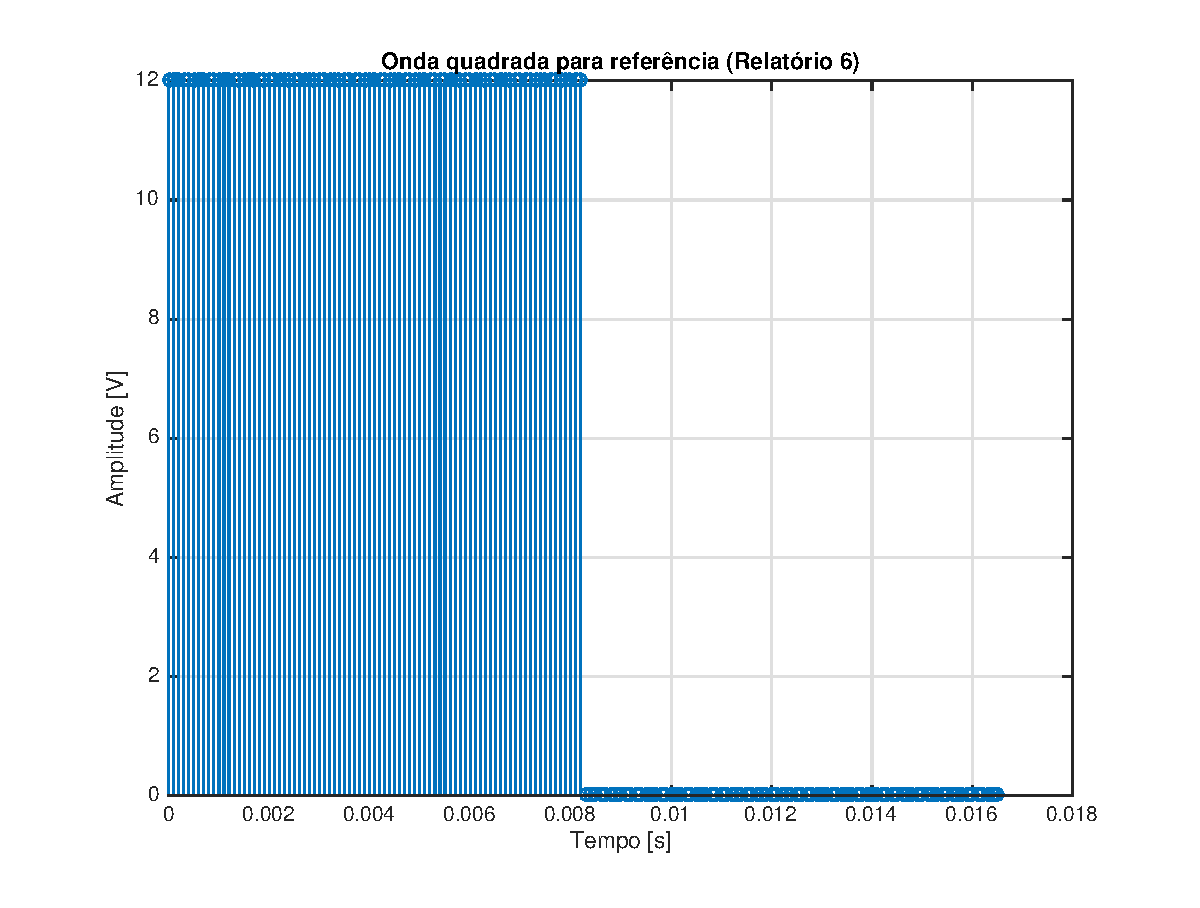
\includegraphics[scale=.45]{Imagens/Relatorio6/quadrada_relatorio6}
  \caption{Sinal de referência, implementado em MATLAB®}
  \label{referencia}
\end{figure}

	Analisa-se pela Figura \ref{referencia} que a onda quadrada tem $12$ Vpp, período de $0,0167$ segundos (configurando em $60$ Hz) e \textit{offset} estabelecido.
	
	 O sistema implementado na Figura \ref{sistemacompleto} é composto pelos seguintes blocos que serão explanados nas seguintes seções subsequentes:
	 
	 \subsection{Circuito de condicionamento de sinais}
	 
	 O sistema que representa o sensor, também apresentado como circuito de condicionamento de sinais, está apresentado na Figura \ref{CCS}.
	 
	 \begin{figure}[hbt]
		\centering
  		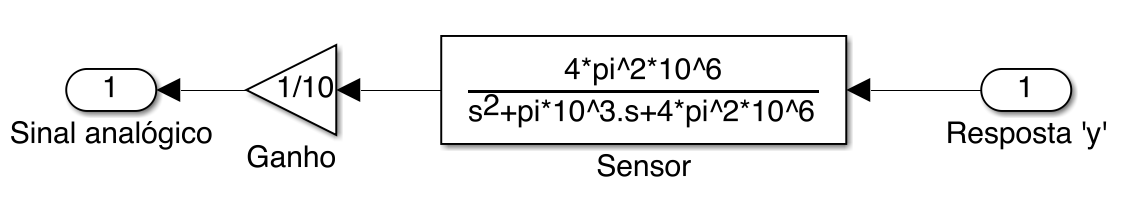
\includegraphics[scale=.4]{Imagens/Relatorio6/Sensor}
  		\caption{Circuito de condicionamento de sinais implementado em Simulink®}
  		\label{CCS}
		\end{figure}
		
		\subsection{ADC de 10 bits}
	 
	 O sistema que representa a inserção do conversor analógico-digital está apresentado na Figura \ref{ADC}.
	 
	 \begin{figure}[hbt]
		\centering
  		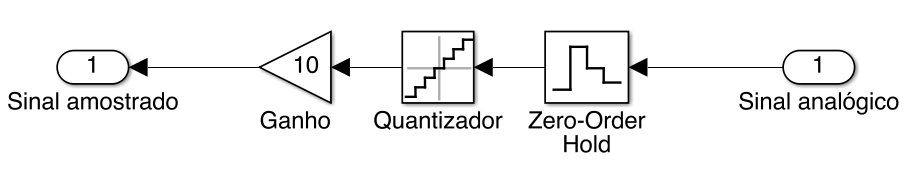
\includegraphics[scale=.4]{Imagens/Relatorio6/ADC}
  		\caption{Sistema que representa a inserção do conversor analógico-digital implementado em Simulink®}
  		\label{ADC}
		\end{figure}
		
		\subsection{Controlador repetitivo}
	 
	 O sistema que representa a aplicação do controlador repetitivo na malha de controle está apresentado na Figura \ref{CRP}.
	 
	 \begin{figure}[hbt]
		\centering
  		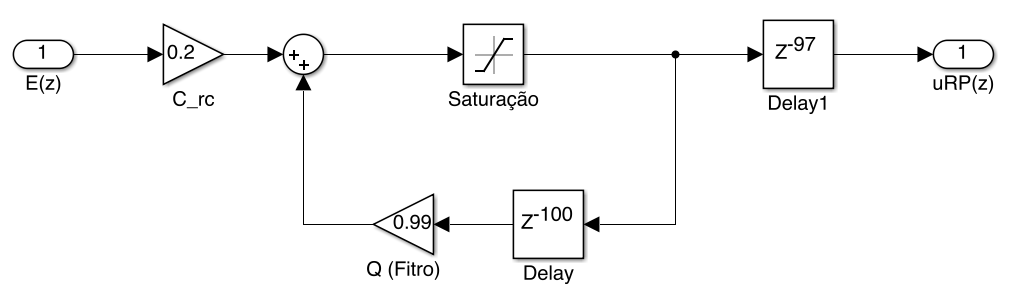
\includegraphics[scale=.4]{Imagens/Relatorio6/Repetitivo}
  		\caption{Sistema que representa a aplicação do controlador repetitivo na malha de controle implementado em Simulink®}
  		\label{CRP}
		\end{figure}
	 
	 \subsection{Proporcional-Integral-Derivativo (PID)}
	 
	 O sistema que representa a aplicação do controlador proporcional-integral-derivativo na malha de controle está apresentado na Figura \ref{PID_6}.
	 
	 \begin{figure}[hbt]
		\centering
  		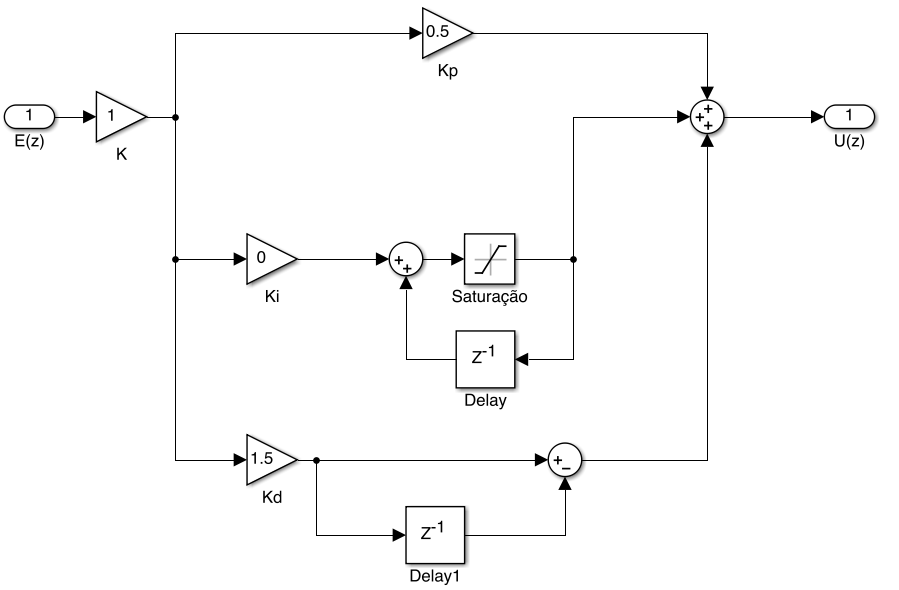
\includegraphics[scale=.45]{Imagens/Relatorio6/PID}
  		\caption{Sistema que representa a aplicação do controlador proporcional-integral-derivativo na malha de controle implementado em Simulink®}
  		\label{PID_6}
		\end{figure}
	 
	 \subsection{PWM}
	 
	 O sistema que representa a criação do sinal PWM está apresentado na Figura \ref{PWM}.
	 
	 \begin{figure}[hbt]
		\centering
  		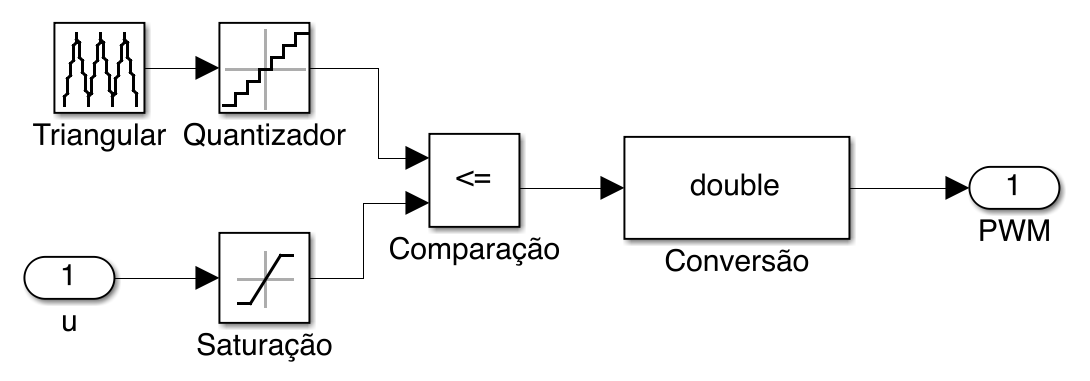
\includegraphics[scale=.4]{Imagens/Relatorio6/PWM}
  		\caption{Circuito para criação de sinal PWM implementado em Simulink®}
  		\label{PWM}
		\end{figure}
		
		O sinal de onda triangular que será utilizado para comparação é apresentado conforme a Figura \ref{triangular}.
		
		\begin{figure}[hbt]
		\centering
  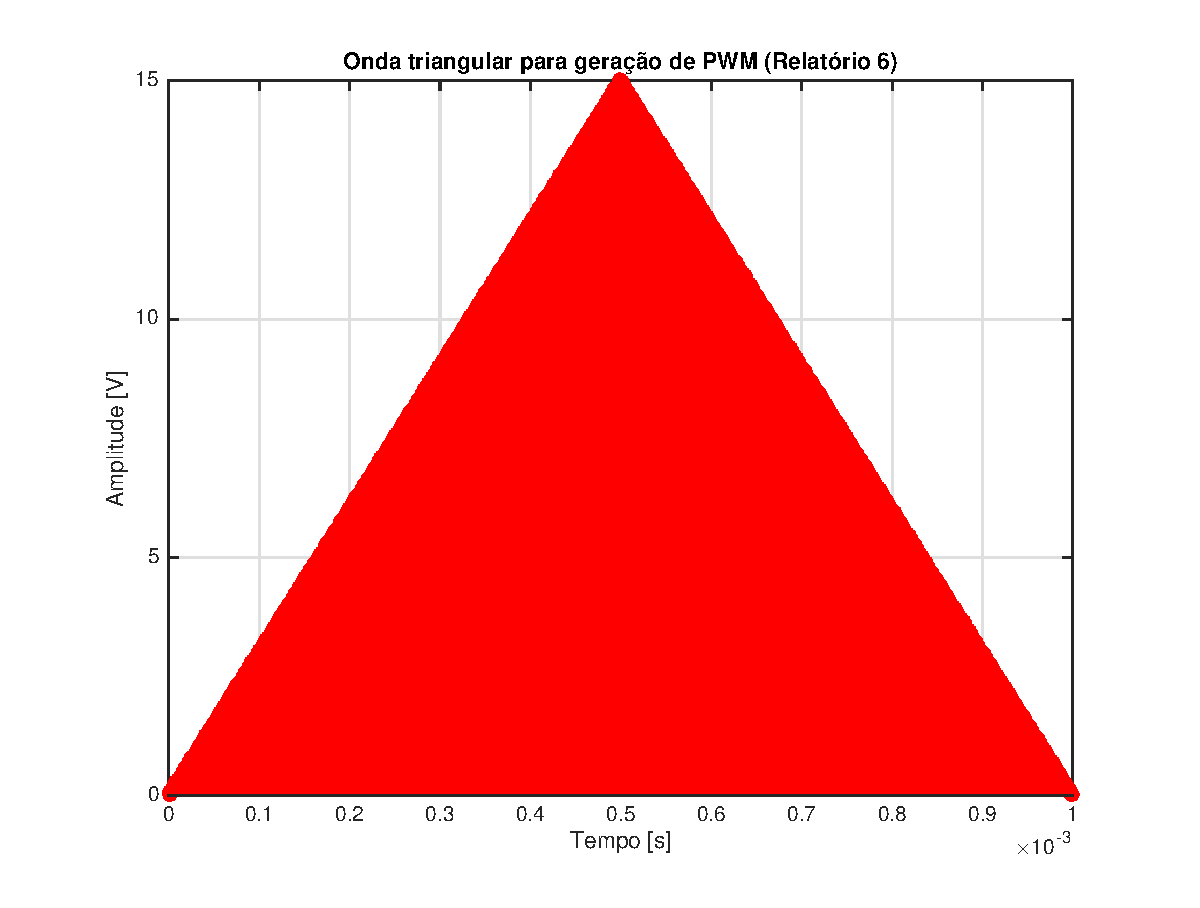
\includegraphics[scale=.45]{Imagens/relatorio6/triangular_relatorio6}
  \caption{Sinal da onda triangular para comparação, implementado em MATLAB®}
  \label{triangular}
\end{figure}

	Percebe-se pela Figura \ref{triangular} que a onda triangular tem amplitude de 15 V e período de 1 ms (Configurando frequência de 1 kHz). 
	 

\section{Resultados e discussões} 